\section{Modelo de domínio}

\begin{figure}[h]
    \centering
    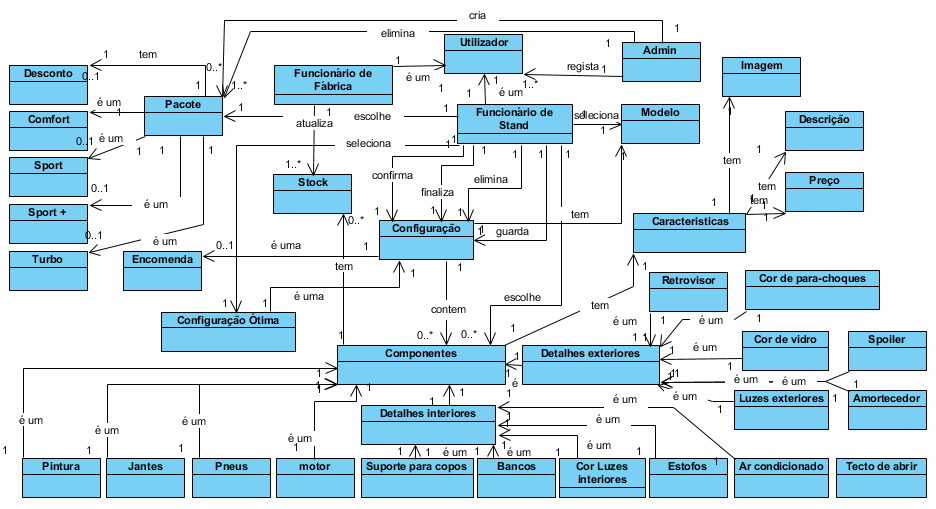
\includegraphics[width=\textwidth]{analise_de_requisitos/img/modelo_de_dominio.png}
    \caption{Modelo de domínio}
    \label{fig:modelo_de_dominio}
\end{figure}


Neste trabalho temos duas classes principais: o funcionário de fábrica e o funcionário de stand. Estes fazem ambos parte da classe \textit{utilizador}, que por sua vez são registados pelo administrador do sistema sempre que necessário adicionar um novo empregado.

O funcionário de stand trata de escolher os componentes das configurações, assim como as confirmações necessárias (se existe stock suficiente) e finalizações (envio de encomendas). Também pode guardar ou eliminar as configurações que pretender, desde que estas não tenham sido finalizadas. Adicionalmente, o funcionário seleciona o modelo do carro a encomendar sempre que iniciar uma nova configuração, pois os componentes diferem de modelo para modelo. Para além da seleção de pacotes inteiros (com desconto), tem a possibilidade de selecionar uma “configuração ótima” que preenche, também automaticamente, os componentes que fazem o melhor uso do limite de dinheiro do respetivo cliente.

Aos funcionários de fábrica, a aplicação permite modificar o stock de cada componente, que atualiza automaticamente no sistema para configurações futuras.

Por fim, para além de puder registar funcionários, o administrador do sistema pode também criar mais pacotes e eliminar os que já existem, conforme as necessidades da fábrica.

\clearpage